\documentclass{beamer}{}
\usepackage[austrian, american]{babel}
\usepackage[T1]{fontenc}
\usepackage[latin1]{inputenc}
\usepackage{algorithm}
\usepackage[noend]{algorithmic}
\usecolortheme{rose}

\title{\huge Federated Learning with TensorFlow~Federated}
\author{Andrea~Hofer, Ignatz~\"Otzlinger, Sabine~Hasenleitner, Kim~Schmider}
\date{}
\begin{document}
    \begin{frame}[plain]
        \maketitle
        \vspace{-.2\textheight}\center
\includegraphics[height=.3\textheight]{img/Tensorflow_logo.png}
    \end{frame}
    \begin{frame} {Introduction}
        \begin{itemize}
            \item Introduction to Machine Learning and Deep Learning
            \item Image Recognition
            \item Why Federated Learning?
            \item CIFAR-10 dataset
            \item Keras
            \item \texttt{FederatedAveraging} Algorithm
        \end{itemize}
    \end{frame}
% Ignatz
    \begin{frame} {What is Machine Learning?}
        \begin{itemize}[<+->]
            \item Big Data: There is no data like more data
            \item Deep Learning: Error rate below 4\%
        \end{itemize}
            \action<+->{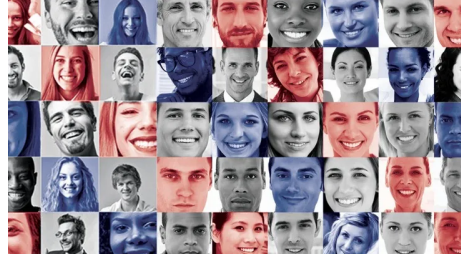
\includegraphics[width=\textwidth]{img/1.png}}
    \end{frame}
    \begin{frame}[plain]
        \center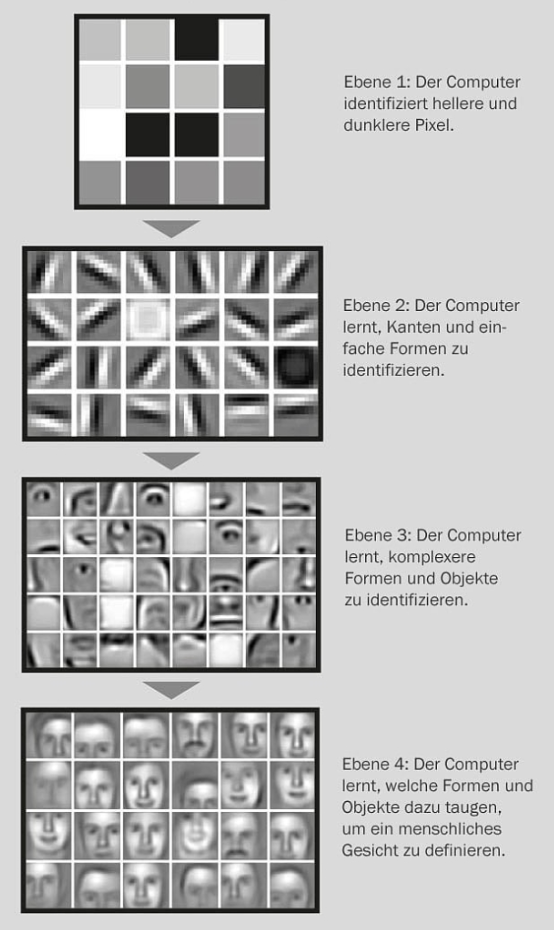
\includegraphics[height=\textheight]{img/4.png}
    \end{frame}
    \begin{frame} {One Neutron}
        \center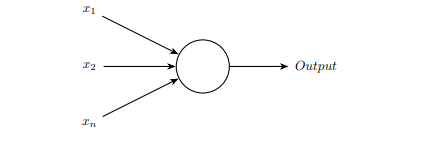
\includegraphics[width=\textwidth]{img/2.png}
    \end{frame}
    \begin{frame} {Neural Network}
        \center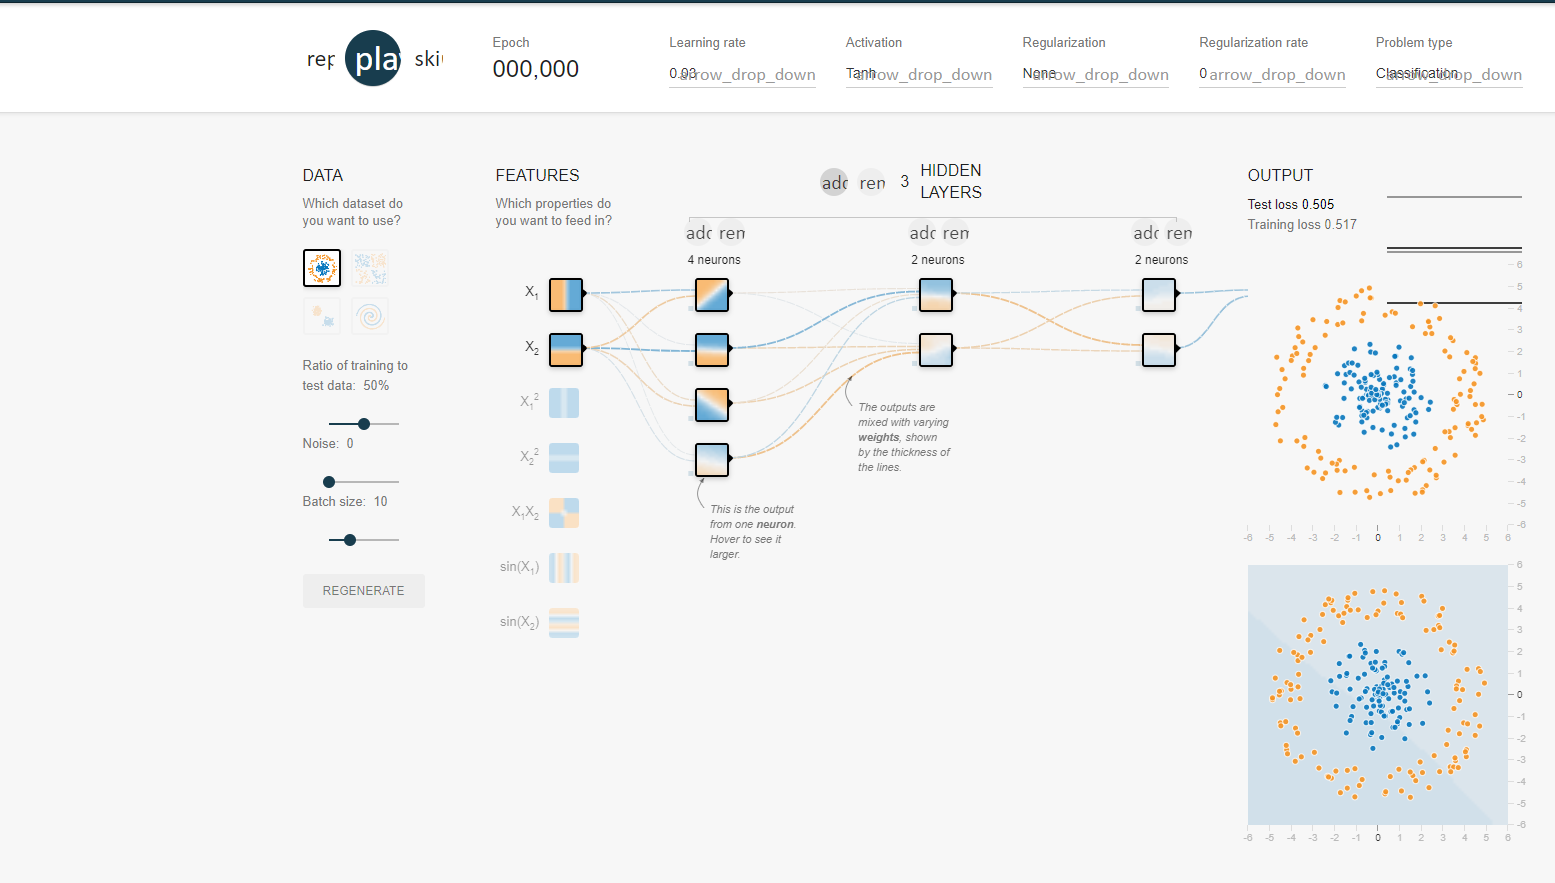
\includegraphics[width=\textwidth]{img/3.png}
    \end{frame}
    \begin{frame} {Deep Learning}
        \center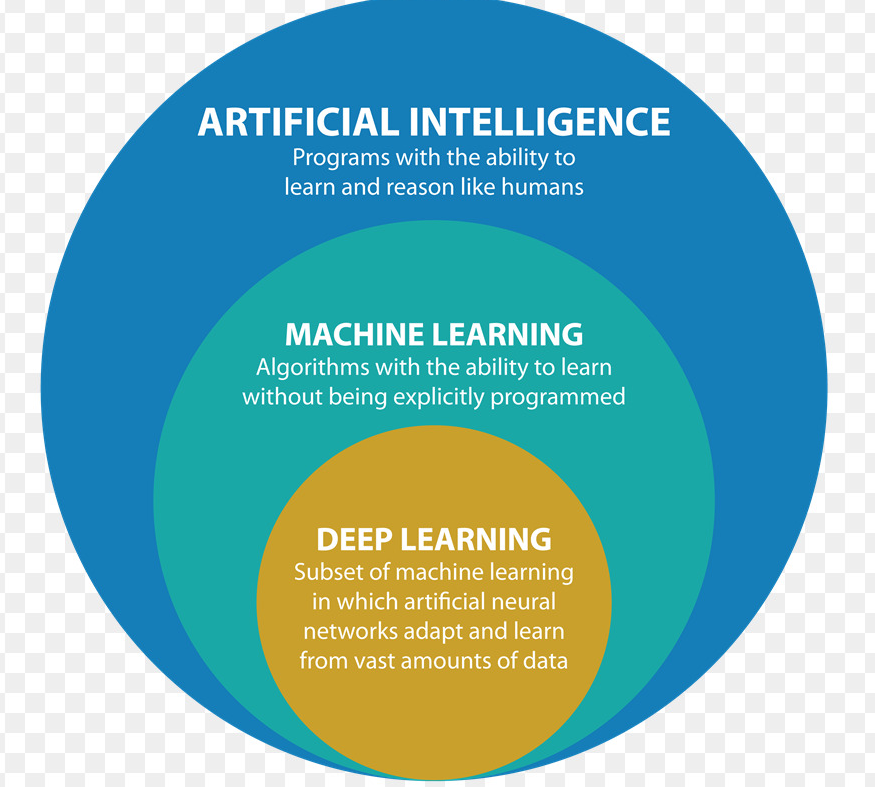
\includegraphics[width=\textwidth]{img/6.png}
    \end{frame}
    \begin{frame} {Text Algorithm is Divided Into Grids of 13x13}
        \center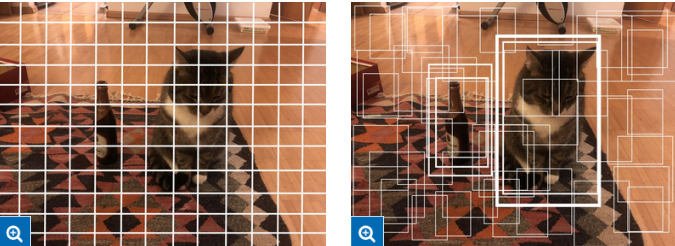
\includegraphics[width=\textwidth]{img/5.png}
    \end{frame}
% Andi    
    \begin{frame} {Image Recognition}
        \begin{itemize}[<+->]
           \item Classification
           \item Object recognition
           \item Instance segmentation
        \end{itemize}
        \begin{center}
            \action<+->{
                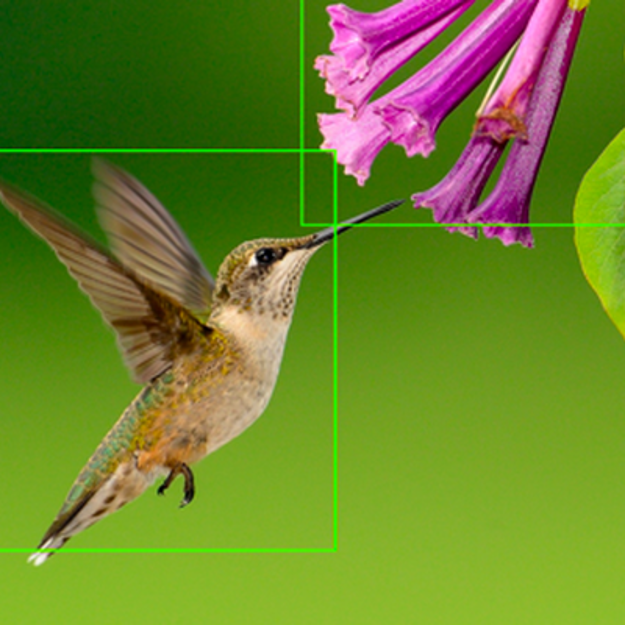
\includegraphics[width=.45\textwidth]{img/bird1.png}
                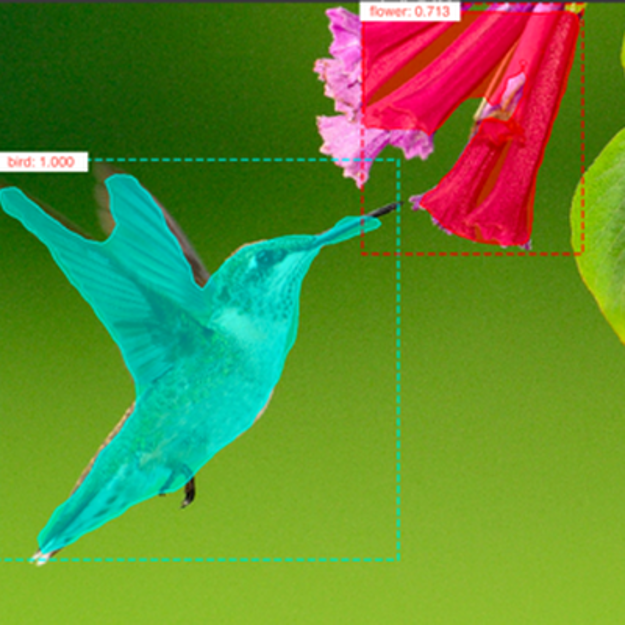
\includegraphics[width=.45\textwidth]{img/bird2.png}
            }
        \end{center}
    \end{frame}
    \begin{frame}[plain]
        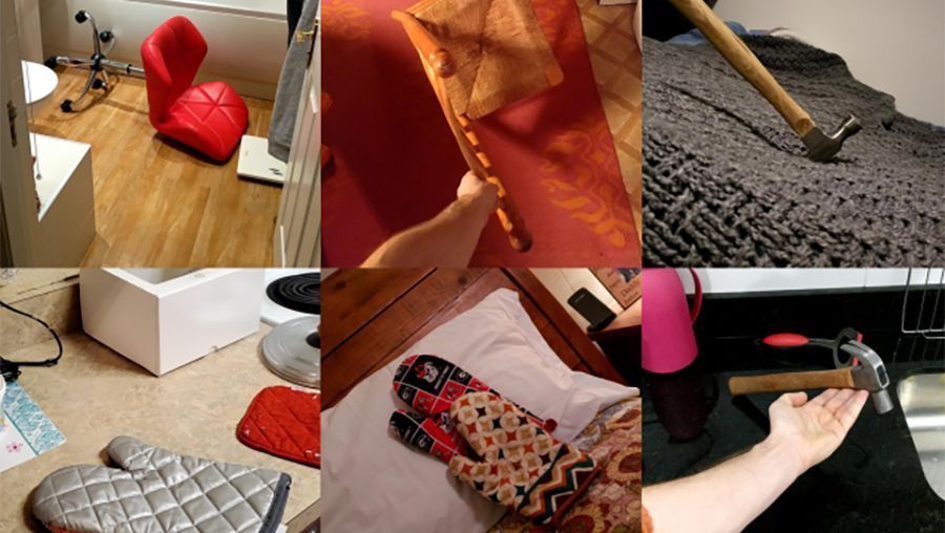
\includegraphics[width=\textwidth]{img/chaos.png}
    \end{frame}
    \begin{frame} {Data Processing with GDPR}
        \begin{itemize}[<+->]
           \item Big data needed, problem with GDPR
           \item Research projects need to stop or cant even start
           \item Solution $\rightarrow$ Federated Learning
        \end{itemize}        
    \end{frame}
    \begin{frame} {Federated Learning}
        \begin{itemize}[<+->]
           \item Calculations on end device
           \item Results of calculations will be sent to global model
           \item Data privacy
        \end{itemize}        
       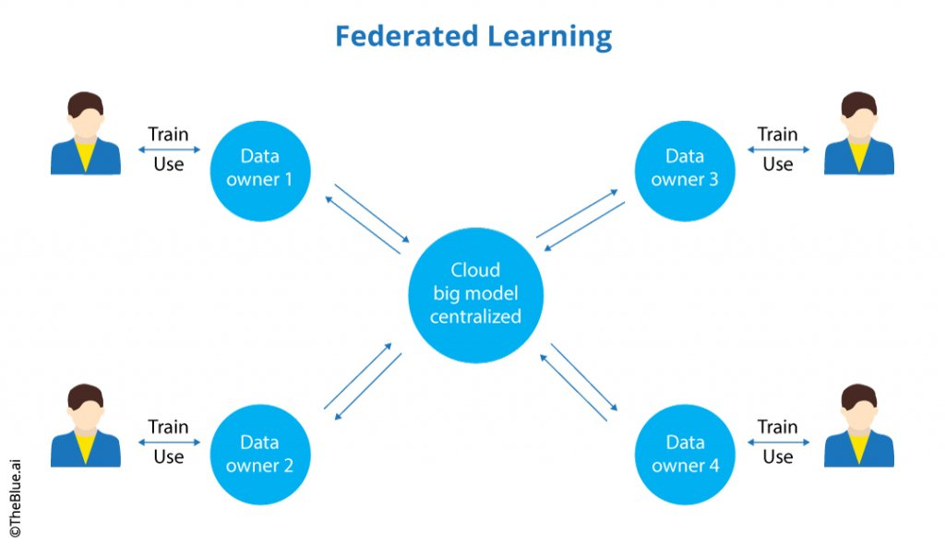
\includegraphics[width=\textwidth]{img/federated-learning.png}%
    \end{frame}
% Sabine
    \begin{frame} {CIFAR-10}
    \begin{itemize}
        \item<+-> CIFAR-10 dataset (Canadian Institute For Advanced Research)
        \item<+-> Collection of images
        \item<+-> Contains 60.000 images
        \item<+-> 10 different classes: 
            \begin{enumerate}
                \item airplanes,
                \item cars,
                \item birds,
                \item cats,
                \item deer,
                \item dogs,
                \item frogs,
                \item horses,
                \item ships,
                \item trucks.
            \end{enumerate}
        \item<+-> 6.000 images per class
        \item<+-> Size 32 x 32
    \end{itemize}
\end{frame}

\begin{frame} {Image Classification}
    \begin{itemize}
        \item How does the image classification work?
        \item \url{https://www.tensorflow.org/tutorials/images/cnn}\\
            This tutorial demonstrates training a simple Convolutional Neural Network (CNN) to classify CIFAR images. (TensorFlow)
    \end{itemize}
\end{frame}

\begin{frame} {KERAS}
    \begin {itemize}[<+->]
        \item Definition as per KERAS Homepage:
            High-level neural networks API, written in Python and capable to running on top of TensorFlow, CNTK, or Theano. It was developed with a focus on enabling fast experimentation. Being able to go from idea to result with the least possible delay is key to doing good research.
            Use Keras if you need a deep learning library that:
        \item Allows for easy and fast prototyping (through user friendliness, modularity, and extensibility)
        \item Supports both convolutional networks and recurrent networks, as well as combinations of the two
        \item Runs seamlessly on CPU and GPU
        \item \url{http://keras.io/}
    \end{itemize}
    \end{frame}

    \begin{frame} {RELU}
    \begin{itemize}
        \item $f(x)=max(0, x)$
    Image from english wikipedia \url{https://en.wikipedia.org/wiki/File:Rectifier_and_softplus_functions.svg}. The file is an original work from user \url{https://en.wikipedia.org/wiki/User:Mcld} (Dan Stowell)
    \end{itemize}
     
    \end{frame}

    \begin{frame} {CIFAR-10}
    \end{frame}

    \begin{frame} {CIFAR-10}
    \end{frame}

    \begin{frame} {CIFAR-10}
    \end{frame}

    \begin{frame} {CIFAR-10}
    \end{frame}
%Kim
    \begin{frame} {Example Uses of Federated Learning}
        \begin{itemize}[<+->]
            \item Medicine
            \item Touch keyboard input prediction
            \item Automatic photo selection
            \item Speech recognition
            \vspace{2em}
            \item With learning based on user interactions labels are directly available
        \end{itemize}
    \end{frame}
    \begin{frame} {Practical Issues With Federated Learning}
        \begin{itemize}[<+->]
            \item Datasets are not representative of population
            \item Data differs from traditional centralized sources
            \item Users' usage styles differ greatly
            \item Many clients each with small datasets
            \item Mobile devices are often offline or on a slow or expensive connection
            \item Time zone differences
        \end{itemize}
    \end{frame}
    \begin{frame} {Resource Utilization}
        \begin{itemize}[<+->]
            \item Data center: Computational costs dominate
            \item Federated Learning: Communication costs dominate
            \item Computation essentially free
            \item Number of updates is minimized:
            \begin{itemize}
                \item by running on more clients in parallel (diminishing returns), or
                \item by performing more computations between updates.
            \end{itemize}
        \end{itemize}
    \end{frame}
    \begin{frame} {\texttt{FederatedAveraging} Algorithm}
        \center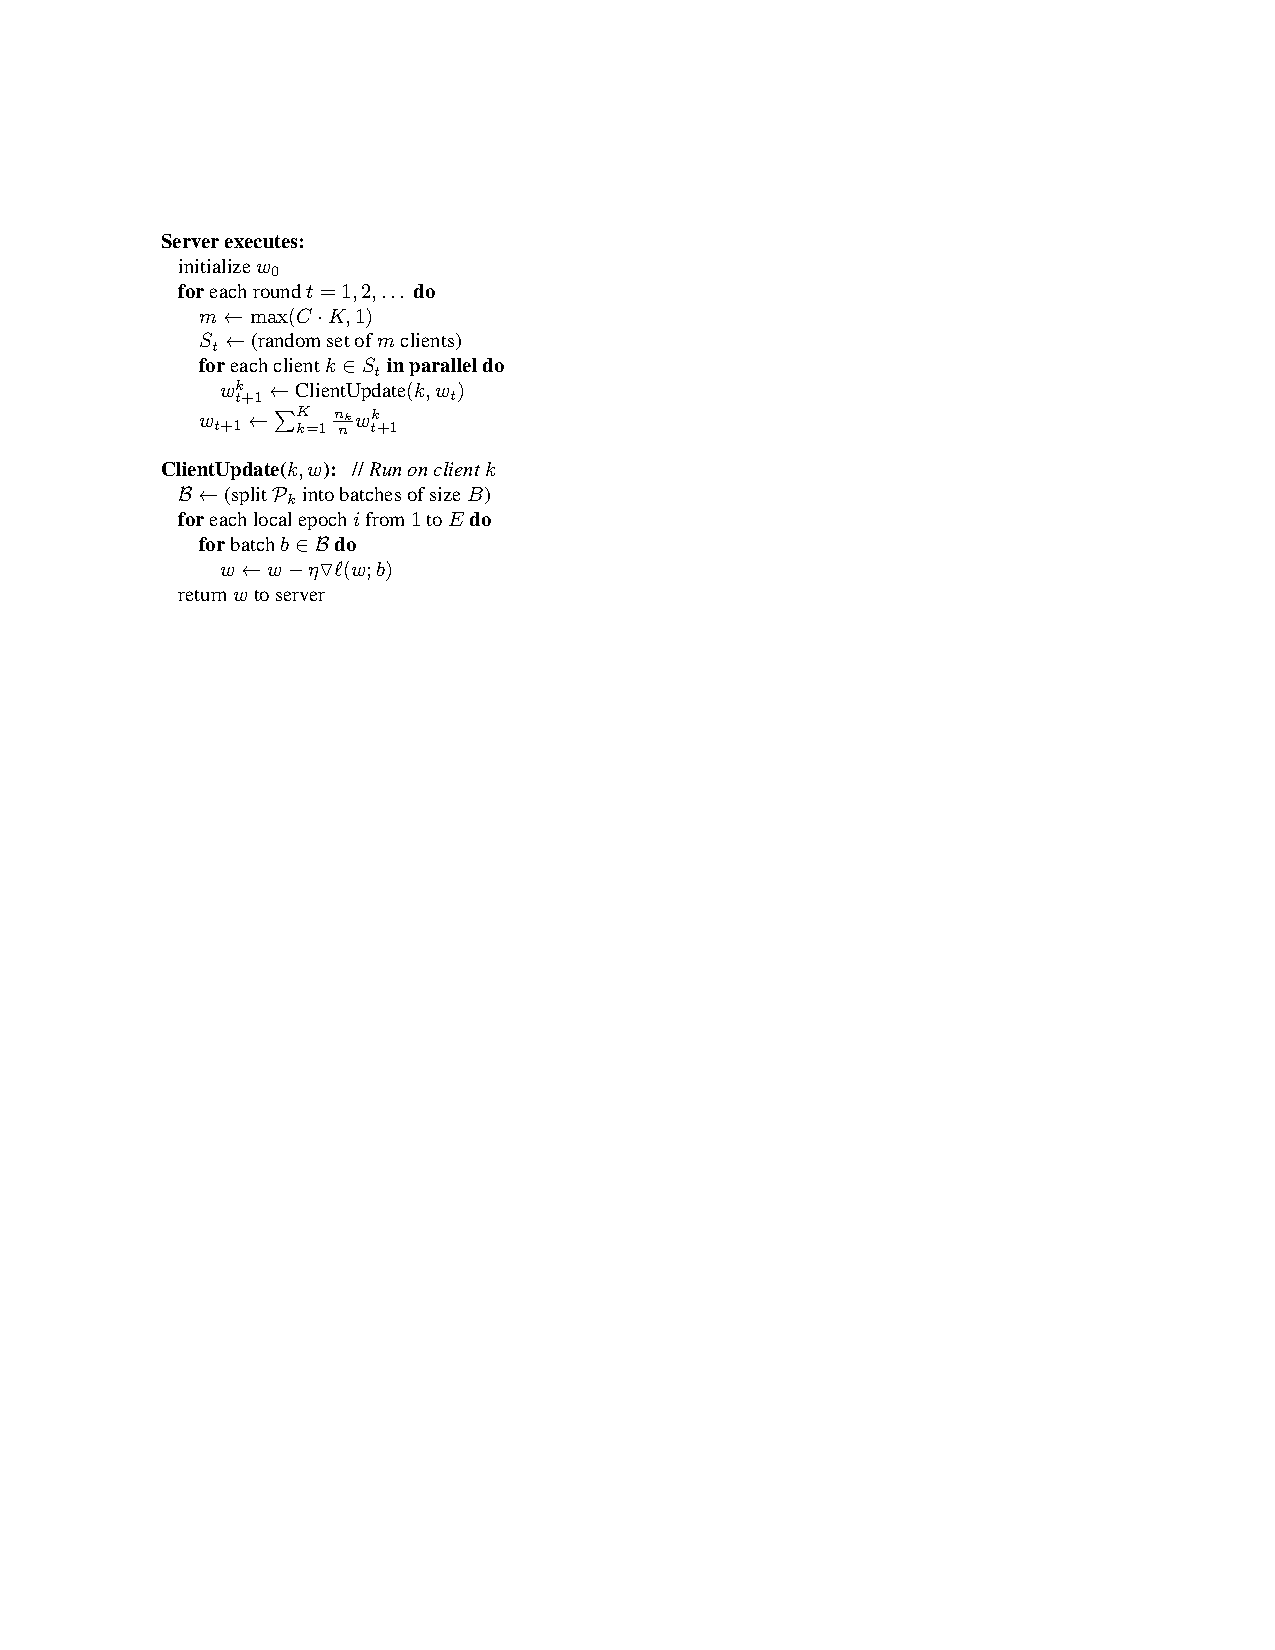
\includegraphics[height=.6\textheight]{img/fedavg.pdf}
    \end{frame}
    \begin{frame}[plain]
        \center{\Huge{Ende}}
    \end{frame}
\end{document}
